% !TEX engine = luatex
% !TeX spellcheck = en_EN

% Copyright (c) 2023, Adam McKellar
%
% This work is licensed under the Creative Commons Attribution-NonCommercial-ShareAlike 4.0 International License. 
% To view a copy of this license, visit http://creativecommons.org/licenses/by-nc-sa/4.0/.


\documentclass{beamer}

\usepackage{amssymb}
\definecolor{commentgreen}{HTML}{006500}
\definecolor{lightgray}{HTML}{d9d9d9}

\usepackage{hyperref}
\hypersetup{
	colorlinks,
	allcolors=.,
	urlcolor=blue,
}

\usepackage{fontspec}
\usepackage{polyglossia}
\setmainlanguage{english}

\usepackage{showexpl}

% https://hartwork.org/beamer-theme-matrix/
\usetheme{Antibes}
\usecolortheme{beaver}
\useinnertheme{circles}

\usepackage[
	type={CC},
	modifier={by-nc-sa},
	version={4.0},
	imagemodifier={-80x15},
]{doclicense}

\usepackage{soul}
\usepackage{listings}

\author{\colorbox{lightgray}{Adam McKellar}}
\title{AIMT4P\quad WebTrans}
\date{\colorbox{lightgray}{11-09-2023}}

\begin{document}
	\setbeamertemplate{background}
	{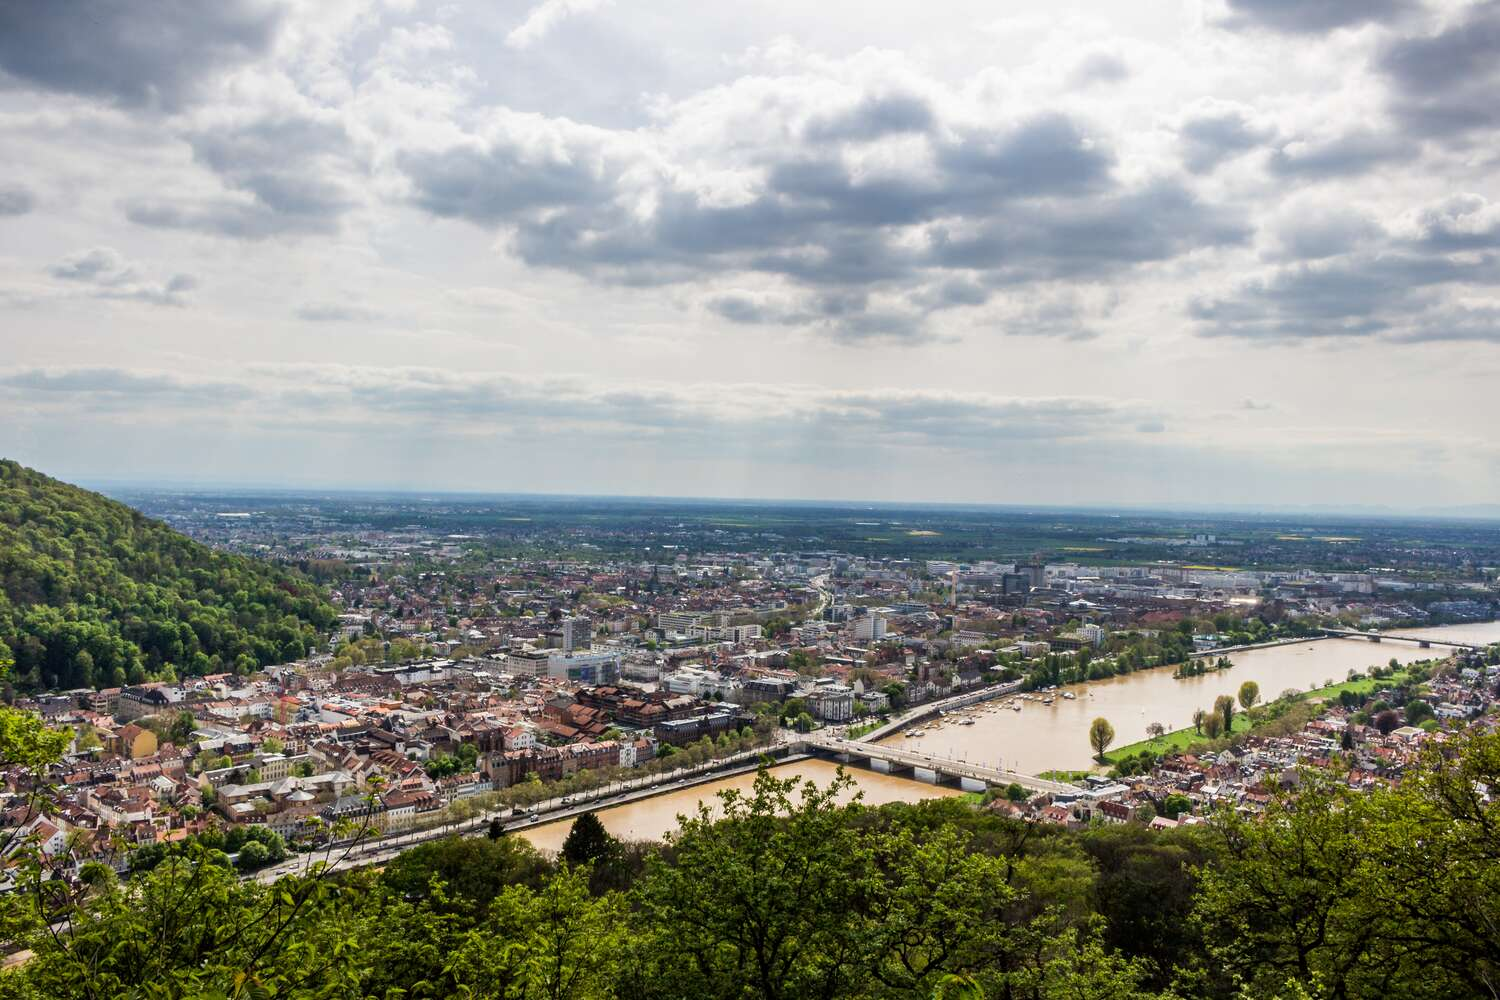
\includegraphics[height=\paperheight,keepaspectratio]{./pictures/background/_MG_1547_s.jpeg}}
	\frame{\titlepage}
	\setbeamertemplate{background}{}
	
	\begin{frame}{Overview}
		\tableofcontents
		\tiny
		\doclicenseThis
	\end{frame}

\section{Introduction}
	\begin{frame}[fragile]{WebTrans: What is the Goal?}
		\only<1->{}
		\only<2->{WebTrans is a Web service to transcode between programming languages.}
		\begin{itemize}
			\item<3-> Accessibility
				\begin{itemize}
					\item WebUI
					\item API
				\end{itemize}
			\item<4-> Back End
				\begin{itemize}
					\item Server
					\item Transcompilation
				\end{itemize}
		\end{itemize}
	\end{frame}


	\begin{frame}[fragile]{Was this Goal archived?}
		\only<1>{}
		\only<2->{Yes \\}
		\begin{itemize}
			\item<3-> Accessibility
				\begin{itemize}
					\item<3-> WebUI
					\item<4-> API
				\end{itemize}
			\item<5-> Back End
				\begin{itemize}
					\item<5-> Docker
					\item<6-> Facebookresearch Transcoder
				\end{itemize}
		\end{itemize}
		\begin{center}
			\includegraphics<3>[width=0.7\linewidth]{pictures/preview_ui/taskcompletion_0.1.1.png}
			\includegraphics<4>[width=\linewidth]{pictures/preview_api/api_create_task.png}
		\end{center}		
	\end{frame}

	\begin{frame}[fragile]{What could not be implemented?}
		\only<1>{}
		\only<2->{Minor Goals}
		\begin{itemize}
			\item<3-> Extending the Transcoder
				\begin{itemize}
					\item<4-> Whole Program Translation
					\item<5-> Speed Up of Translation
				\end{itemize}
			\item<6-> Administrative Tools
				\begin{itemize}
					\item<7-> Self hosted Statistics
					\item<8-> Statistics through Trackers
					\item<9-> Built in abuse and security monitoring
				\end{itemize}
		\end{itemize}
	\end{frame}

\section{Implementation}
	\begin{frame}[fragile]{How was the Goal archived?}
		\only<+>{}
		\only<+>{Programming}
		\only<+->{Docker}
		\begin{itemize}[<+->]
			\item Packaging the Applications
				\begin{itemize}
					\item Transcoder
					\item Major Task
					\item Problem Preview: hardcoded paths
				\end{itemize}
			\item Docker Compose
				\begin{itemize}
					\item Splitting up Applications
						\begin{itemize}
							\item DB - WebUI - Transcoder
						\end{itemize}
					\item Easy Deployment
				\end{itemize}
		\end{itemize}
	\end{frame}
	\begin{frame}[fragile]{How was the Goal archived?}
		Lucky Web Framework
		\begin{itemize}[<+->]
			\item Crystal
				\begin{itemize}
					\item Compiled \& Gc
					\item Tags for HTML
					\item Transpilable into JS
					\item \color{red} Red Flag \color{black}
					\begin{itemize}
						\item \color{red} Crystal compilation takes ages. \checkmark \color{black}
						\item \color{red} GUI development is in Crystal. \checkmark \color{black}
					\end{itemize}
				\end{itemize}
			\item No builtin Reactivity
				\begin{itemize}
					\item Static Content
					\item Modules \& Conditional Rendering
					\item ORM handles forms
					\item Vanilla JS \--- React JS \--- Vue JS
				\end{itemize}
			\item 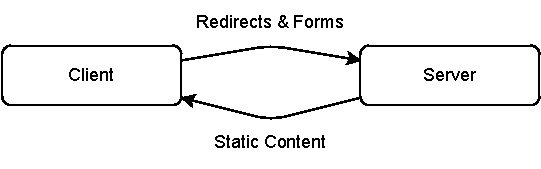
\includegraphics[height=0.25\textheight]{pictures/client_server/interaction.pdf}
		\end{itemize}		
	\end{frame}

	\begin{frame}[fragile]{What is the Code Quality?}
		\begin{itemize}[<+->]
			\item Docker
				\begin{itemize}
					\item Many parallel building stages
					\item Naming of building stages spontaneous \(\Rightarrow\) similar
					\item \(\Rightarrow\) Slightly chaotic looking
					\item Documentation: Why is library xyz installed?
					\item \(\Rightarrow\) Room for improvement
				\end{itemize}
			\item Lucky
				\begin{itemize}
					\item Overly complex default file structure
					\item HTML in Crystal
					\item Too many files
				\end{itemize}
			\item Testing
				\begin{itemize}
					\item No Unit Tests
					\item Cumbersome System Testing
				\end{itemize}
		\end{itemize}
	\end{frame}

\section{Difficulties}
	\begin{frame}[fragile]{What where special difficulties?}
		Packaging the Transcoder
		\begin{itemize}[<+->]
			\item Slow Debugging \(\Leftarrow\) Long Build Times
			\item Major Flaws in Transcoder an Libraries
			\begin{itemize}
				\item Many libraries are not maintained \textit{(fastBPE >:| )}
				\item Year old Bugs \textit{(fastBPE >:| )}
				\item Hard coded Paths and Names \textit{(the transcoder)}
				\item Unhelpful Messages \textit{(the transcoder \& fastBPE)}
			\end{itemize}
		\end{itemize}
	\end{frame}
	\begin{frame}[fragile]{What where special difficulties?}
		Missing Documentation
		\begin{itemize}[<+->]
			\item Crystal is not well documented.
				\begin{itemize}
					\item Confusing website layout.
					\item Functions are not well enough explained.
					\item Explanation of attributes is missing.
					\item No examples for usage of function give.
					\item Searching the web for "crystal lang" problems more often than not results in "crystal reports" questions.
				\end{itemize}
			\item Lucky has not enough examples and is lacking clear documentation.
				\begin{itemize}
					\item How to reach interactive web pages is not described.
					\item For major features there is a lack of extensive examples.
					\item Examples for using HTML forms are not under \textit{HTML Forms} but under \textit{Database}...
				\end{itemize}
		\end{itemize}
	\end{frame}
	\begin{frame}[fragile]{What where special difficulties?}
		Bugs
		\begin{itemize}[<+->]
			\item module 'fastBPE' has no attribute 'fastBPE'
				\begin{itemize}
					\item Latest installer script does not work for my docker image.
					\item PyPi package does not work when trying to install it with "pip install -r requirements.txt"
					\item Solution: Brute force every possible way to install
					\item => "pip install fastBPE" somehow works \--- Why tho?
				\end{itemize}
			\item Crystal "Process.run"
				\begin{itemize}
					\item Actually costed me hours to fix.
					\item System dependent bug.
					\item "Process.run" only writes to "output" if "error" is also listened on \&\& on that docker file \&\& with that program.
					\item \color{red} "Process.run(python\_exec, exec\_params, env: {"PATH" => ENV["PATH"]}, input: input, output: output)"
					\item \color{green} "Process.run(python\_exec, exec\_params, env: {"PATH" => ENV["PATH"]}, input: input, output: output, error: err)" \color{black}
				\end{itemize}
		\end{itemize}
	\end{frame}
	\begin{frame}[fragile]{What where special difficulties?}
		Bugs
		\begin{itemize}
			\item Debugging the Style of the web page is tedious.
			\begin{itemize}[<+->]
				\item HTML and classes written in crystal
				\item \(\Rightarrow\) Long compiles times
				\item No interactive UI development
			\end{itemize}
		\end{itemize}
	\end{frame}

	\begin{frame}[fragile]{Were they solvable?}
		UI is lacking
		\begin{itemize}
			\item Missing Footer
			\item Button if inserted then also goes missing.
		\end{itemize}
	\end{frame}

	\begin{frame}[fragile]{What did I learn from this?}
		\only<+>{}
		\only<+->{Polished and well documented tools are key.}
		\only<+->{
			\begin{itemize}
				\item Rust
				\item WASM
				\item Leptos
			\end{itemize}
		}		
	\end{frame}

\section{Closure}
	\begin{frame}[fragile]{Project Demo}
		Demo here
	\end{frame}

	\begin{frame}[fragile]{Links}
		\begin{itemize}
			\item Main Public Repo: \url{https://github.com/WyvernIXTL/webtrans}
			\item Private Repo: \url{https://github.com/pvs-hd-tea/23ss-WebTrans}
			\item Private Release with prebuilt docker images and presentation: \url{https://github.com/pvs-hd-tea/23ss-WebTrans/releases/tag/0.1.1}
			\item WebUI Documentation: \url{https://wyvernixtl.github.io/webtrans/}
		\end{itemize}
	\end{frame}
		
	
\end{document}